%%%%%%%% mlsys 2022 EXAMPLE LATEX SUBMISSION FILE %%%%%%%%%%%%%%%%%
\documentclass{article}


% if you need to pass options to natbib, use, e.g.:
\PassOptionsToPackage{round}{natbib}
% before loading neurips_2022


% ready for submission
\usepackage{neurips_2022}

\usepackage{enumitem}
% to compile a preprint version, e.g., for submission to arXiv, add add the
% [preprint] option:
% \usepackage[preprint]{neurips_2022}


% to compile a camera-ready version, add the [final] option, e.g.:
%     \usepackage[final]{neurips_2022}


% to avoid loading the natbib package, add option nonatbib:
% \usepackage[nonatbib]{neurips_2022}


\usepackage[utf8]{inputenc} % allow utf-8 input
\usepackage[T1]{fontenc}    % use 8-bit T1 fonts
\usepackage{hyperref}       % hyperlinks
\usepackage{url}            % simple URL typesetting
\usepackage{booktabs}       % professional-quality tables
\usepackage{amsfonts}       % blackboard math symbols
\usepackage{nicefrac}       % compact symbols for 1/2, etc.
\usepackage{microtype}      % microtypography
\usepackage{xcolor}         % colors
\usepackage{graphicx}
\usepackage{subfigure}
\usepackage{bm}
\usepackage{amsmath,amssymb}
\usepackage{algorithm}
\usepackage[noend]{algpseudocode}
\usepackage{soul}
\usepackage{xspace}
\usepackage{multirow}
\usepackage{makecell}
\usepackage{ulem}

\DeclareMathOperator{\round}{round}
\DeclareMathOperator{\clamp}{clamp}

\newcommand{\R}{\mathbf R}
\newcommand{\Z}{\mathbf Z}
\newcommand{\cin}{C_{\text{in}}}
\newcommand{\cout}{C_{\text{out}}}
\newcommand{\wb}{\mathbf W}
\newcommand{\xb}{\mathbf x}
\newcommand{\yb}{\mathbf y}
\newcommand{\calA}{\mathcal{A}}
\newcommand{\bz}{\mathbf{z}}
\newcommand{\bv}{\mathbf{v}}
\newcommand{\bx}{\mathbf{x}}
\newcommand{\ba}{\mathbf{a}}
\newcommand{\calZ}{\mathcaL{Z}}
\newcommand{\SecInd}{{\sc SecInd}\xspace}
\newcommand{\SecAgg}{{\sc SecAgg}\xspace}
\newcommand{\FedAvg}{{\sc FedAvg}\xspace}
\newcommand{\SGD}{{\sc SGD}\xspace}

\def\ie{\textit{i.e.,}\@\xspace}
\def\eg{\textit{e.g.,}\@\xspace}

\newcommand{\pierre}[1]{{\color{purple}Pierre: #1}}
\newcommand{\sayan}[1]{{\color{red}Sayan: #1}}
\newcommand{\karthik}[1]{{\color{blue}Karthik: #1}}
\newcommand{\graham}[1]{{\color{green}Graham: #1}}
\newcommand{\ilya}[1]{{\color{red}Ilya: #1}}
\newcommand{\ashkan}[1]{{\color{blue}Ashkan: #1}}
\newcommand{\dzmitry}[1]{{\color{purple}Dzmitry: #1}}
\newcommand{\modif}[1]{{\color{black}#1}}

\title{Reconciling Security and Communication Efficiency in Federated Learning}
% Communication Efficient and Secure Federated Learning
% Unifying Secure Federated Learning and Communication Efficiency
% The Missing Bit for Practical Efficient Communication in Federated Learning
% Enabling Federated Learning with Communication Efficiency


% The \author macro works with any number of authors. There are two commands
% used to separate the names and addresses of multiple authors: \And and \AND.
%
% Using \And between authors leaves it to LaTeX to determine where to break the
% lines. Using \AND forces a line break at that point. So, if LaTeX puts 3 of 4
% authors names on the first line, and the last on the second line, try using
% \AND instead of \And before the third author name.


\author{
Karthik Prasad\thanks{Equal contribution. Correspondence to \texttt{pstock@fb.com}.} $^{~\dagger}$~~ Sayan Ghosh\footnotemark[1]$^{~~\dagger}$~~ Graham Cormode$^\dagger$~~ \\ \textbf{Ilya Mironov$^\dagger$~~ Ashkan Yousefpour$^\dagger$~~ Pierre Stock$^\dagger$} \\ $^\dagger$Meta AI
%   David S.~Hippocampus\thanks{Use footnote for providing further information
%     about author (webpage, alternative address)---\emph{not} for acknowledging
%     funding agencies.} \\
%   Department of Computer Science\\
%   Cranberry-Lemon University\\
%   Pittsburgh, PA 15213 \\
%   \texttt{hippo@cs.cranberry-lemon.edu} \\
  % examples of more authors
  % \And
  % Coauthor \\
  % Affiliation \\
  % Address \\
  % \texttt{email} \\
  % \AND
  % Coauthor \\
  % Affiliation \\
  % Address \\
  % \texttt{email} \\
  % \And
  % Coauthor \\
  % Affiliation \\
  % Address \\
  % \texttt{email} \\
  % \And
  % Coauthor \\
  % Affiliation \\
  % Address \\
  % \texttt{email} \\
}


\begin{document}

\maketitle 

\begin{abstract}

Cross-device Federated Learning is an increasingly popular machine learning setting to train a model by leveraging 
a large population of client devices with high privacy and security guarantees. 
However, 
communication efficiency remains a major bottleneck when scaling federated learning to production environments, particularly due to bandwidth constraints during uplink communication.
In this paper, we formalize and address the problem of compressing client-to-server model updates
under the Secure Aggregation primitive, a core component of Federated Learning pipelines that allows the server to aggregate the client updates without accessing them individually. 
In particular, we adapt standard scalar quantization and pruning methods
to Secure Aggregation and propose Secure Indexing, a variant of Secure Aggregation that supports quantization for extreme compression.
We establish state-of-the-art results on LEAF benchmarks in a secure Federated Learning setup with up to 40$\times$ compression in uplink communication 
with no meaningful loss in utility compared to uncompressed baselines.
% compared to a.
% \karthik{\st{with less than one bit per weight on the LEAF benchmark and no significant loss in utility.}} 
% \karthik{I have edited the abstract a bit, please check history to review my changes}
\end{abstract}

% this must go after the closing bracket ] following \twocolumn[ ...

% This command actually creates the footnote in the first column
% listing the affiliations and the copyright notice.
% The command takes one argument, which is text to display at the start of the footnote.
% The \mlsysEqualContribution command is standard text for equal contribution.
% Remove it (just {}) if you do not need this facility.

\section{Introduction}
\label{sec:intro}

Federated Learning (FL) is a distributed machine learning (ML) paradigm that trains a model across a number of participating entities holding local data samples.
% , without exchanging them. 
In this work, we focus on \emph{cross-device} FL that harnesses a large number (up to hundreds of millions) of edge devices with disparate characteristics such as availability, compute, memory, or connectivity
resources~\citep{kairouz2019advances}. %that harnesses potential
% Current applications of FL are designed to scale up to client populations of hundreds of millions or even billions. 
Two challenges to the success of cross-device FL are privacy and scalability. 
FL was originally motivated for improving privacy since data points remain on client devices. 
% and only small model updates were shared to a co-ordinating server.
However, as with other forms of ML, information about training data can be extracted via membership inference or reconstruction attacks on a trained model \citep{carlini2021membership,carlini2020extracting}, or leaked through local updates~\citep{MelisSCS19,geiping2020inverting}. 
Consequently, Secure Aggregation (\SecAgg) protocols were introduced to prevent the server from directly observing individual client updates, which is a major vector for information leakage~\citep{bonavitz2019federated,huba2021papaya}. 
Additional mitigations such as  Differential Privacy (DP) may be required to offer further protection 
against attacks~\citep{dwork2006calibrating,abadi2016deep}, as discussed in Section~\ref{sec:discussion}.
% , as discussed in Section~\ref{sec:discussion}.
%As an additional layer of protection against statistical inference attacks, SecAgg is usually paired with Differential Privacy (DP) \citep{dwork2006calibrating}. To realize the full promise of FL as a privacy-enhancing technology, we need both SecAgg and Differential Privacy.

Ensuring scalability to populations of heterogeneous clients is the second challenge for FL.
% There are many aspects for FL scalability, such as ensuring that model updates can be calculated efficiently 
% by devices with various capabilities and intermittent availability~\citep{bonavitz2019federated}.
% Here, we focus on the communication bottleneck as the primary concern.
Indeed, wall-clock training times are highly correlated with increasing model and batch sizes~\citep{huba2021papaya}, even with recent efforts such as FedBuff~\citep{nguyen2021federated},
% With increasing model and batch sizes, the wall-clock training time increases accordingly~\citep{huba2021papaya}. 
% Despite efforts such as buffered asynchronous aggregation~\cite{nguyen2021federated}, 
and communication overhead between the server and clients dominates model convergence time.
% cross-device FL remains bottlenecked by communication latency between the server and the clients. 
% \karthik{should we mention this paper in a different way? Fedbuff paper doesn't explicitly call out latency as an issue, nor do we run experiments to on async fl ourselves}  \ashkan{I also think the transition can be smoother: first we focus on scalability and billions. Then we say communication is the bottleneck} 
Consequently, compression techniques were used to reduce the communication bandwidth while maintaining model accuracy.
However, a fundamental problem has been largely overlooked in the literature: in their native form, standard compression methods such as scalar quantization and pruning are not compatible with \SecAgg. 
This makes it challenging to ensure both security and communication efficiency.
% at the same time.
% the default method to provide security for client update, 
% presenting an unpleasant dichotomy between security or efficiency. 


% Second, this is the most restricted direction, since upload bandwidth remains more restricted than download. 
% In the US, fixed-line broadband speeds typically achieve a ratio of $3\times$ to $20\times$ more download bandwidth than upload
% bottlenecks remain, and so we seek to reduce the message size of clients by \textit{compression}. 
% Compression has been widely proposed in various ML scenarios, in the form of pruning (removing model parameters) and quantization (reducing fidelity of parameter representation). 
% Indeed, these techniques have been successfully used in FL settings with appreciable improvements in communication while maintaining model accuracy. 
% However, there is a fundamental problem which has been largely overlooked in the literature: in their native form, these compression methods are not compatible with SecAgg, the default method to provide security for client updates. 
% This presents an unpleasant dichotomy: we can have security or efficiency, but not both. 
%
%
% In this paper, we resolve this gap by showing how to modify FL compression techniques to make them security-friendly. We focus on compressing \emph{uplink} updates from clients to the server for two reasons. 
% First, uplink communications are subject to Secure Aggregation protocols to ensure a high security bar, while downlink updates broadcasted by the server are deemed public. 
% Second, upload bandwidth is generally more restricted than download. For instance, according to the most recent FCC report, the ratio of download to upload speeds for DSL/cable providers\footnote{Fixed-line broadband is most relevant since FL is typically restricted to using unmetered connections, usually over Wi-Fi~\citep{huba2021papaya}.} in the US ranges between 3$\times$ to 20$\times$~\citep{fcc-broadband}.
% % This requires some meticulous changes to coordinate clients to use the same global (non-private) hyperparameters, and show that this coordination does not damage model quality. 
% % For the strongest compression methods, we step outside of the SecAgg primitive and propose a new secure primitive, Secure Indexing, which enables the best compression ratios without sacrificing utility. 
% Finally, efficient and secure uplink communication brings several benefits beyond speeding up convergence: 
% lowering communication cost reduces selection bias due to undersampling clients with limited connectivity, improving fairness and inclusivity metrics. 
% It also shrinks the carbon footprint of FL, whose fraction attributable to communication can reach 95\%~\citep{qiu2021first}.
%
%In this paper, w
We address this gap by adapting compression techniques to make them compatible with \SecAgg. We focus on compressing \emph{uplink} updates from clients to the server for three reasons. 
First, uplink communication is more sensitive and so is subject to a high security bar, whereas downlink updates broadcast by the server are deemed public. 
Second, upload bandwidth is generally more restricted than download bandwidth. For instance, according to 
a recent FCC report, 
%the most recent \modif{FCC\footnote{\modif{US Federal Communications Commission.}} report}, 
the ratio of download to upload speeds for DSL and cable providers\footnote{FL is typically restricted to using unmetered connections, usually over Wi-Fi~\citep{huba2021papaya}.} in the US ranges between 3$\times$ to~20$\times$~\citep{fcc-broadband}.
% Fixed-line broadband is most relevant since
% This requires some meticulous changes to coordinate clients to use the same global (non-private) hyperparameters, and show that this coordination does not damage model quality. 
% For the strongest compression methods, we step outside of the SecAgg primitive and propose a new secure primitive, Secure Indexing, which enables the best compression ratios without sacrificing utility. 
Efficient uplink communication brings several benefits beyond speeding up convergence: 
lowering communication cost reduces selection bias due to under-sampling clients with limited connectivity, improving fairness and inclusiveness. 
It shrinks the carbon footprint of FL, the fraction of which attributable to communication can reach 95\%~\citep{qiu2021first}.
In summary, we present the following contributions: 
\begin{itemize}
    \item We highlight the fundamental mismatch between two critical components of the FL stack: \SecAgg protocols and uplink compression mechanisms.
    
    \item We formulate solutions by imposing a linearity constraint on the decompression operator, as illustrated in Figure~\ref{fig:secagg_summary} in the case of TEE-based \SecAgg.
    
    \item We adapt the popular scalar quantization and (random) pruning compression methods for compatibility with the FL stack that require no changes to the \SecAgg protocol.
    
    \item For extreme uplink compression without compromising security, we propose Secure Indexing (\SecInd), a variant of \SecAgg that supports product quantization. %and admits a secure implementation.
\end{itemize}

\begin{figure*}[t]
    \centering
    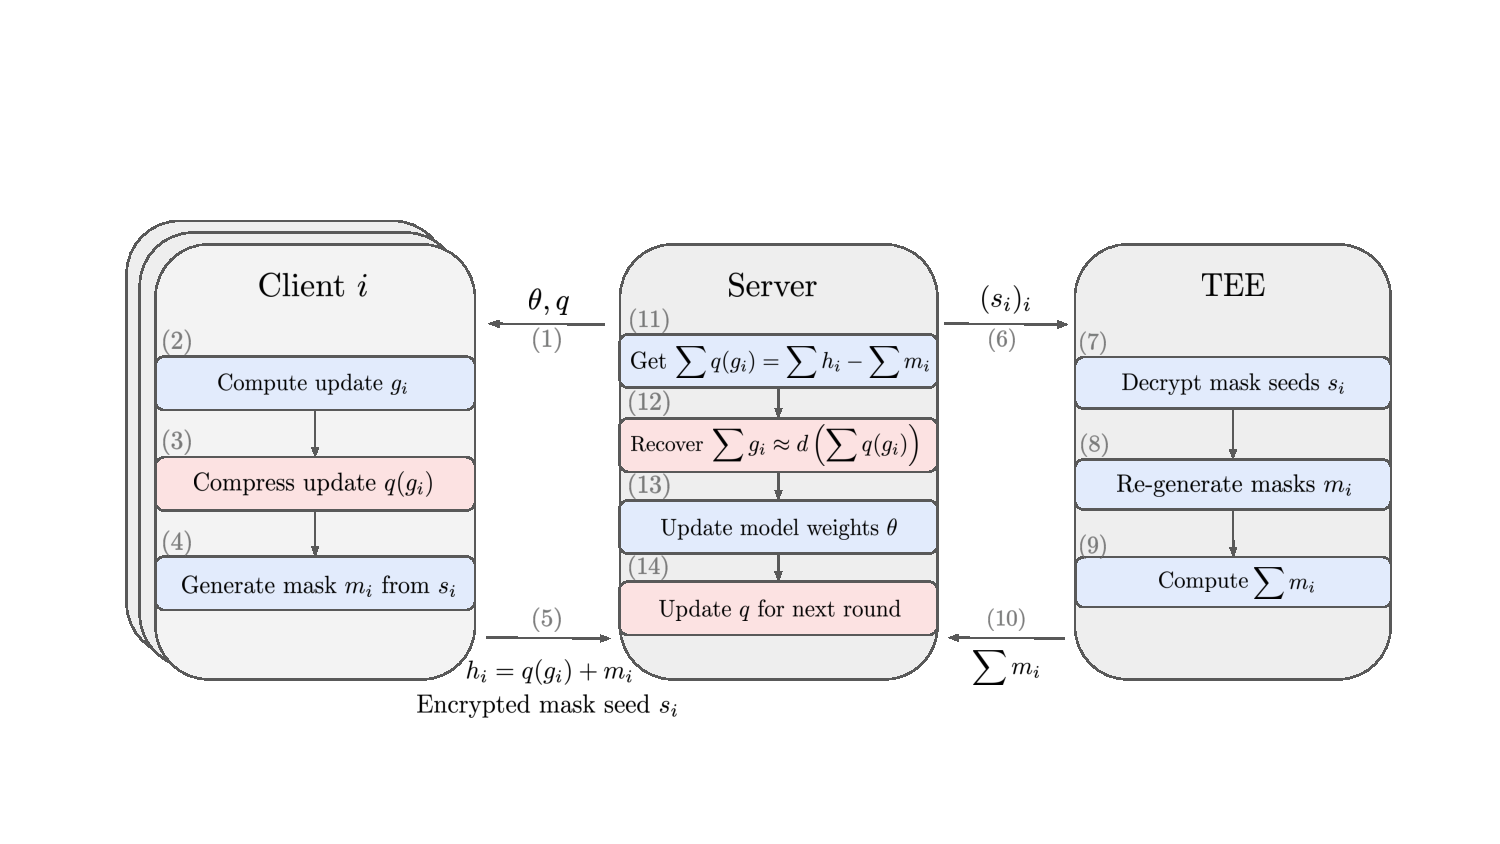
\includegraphics[width=0.8\textwidth]{figs/secagg_summary_new.pdf}
    %\vspace{-5mm}
    \caption{\label{fig:secagg_summary}
    Summary of the proposed approach for one FL round, where we omit the round dependency and \modif{Differential Privacy (DP)} for clarity. Blue boxes denote standard steps and red boxes denote additional steps for uplink compression. Client $i$ computes local model update $g_i$, compresses it with the compression operator $q$, and encrypts it by adding a random mask $m_i$ in the compressed domain, hence reducing the uplink bandwidth (steps 2--4). The server recovers the aggregate in the compressed domain by leveraging any \SecAgg protocol \modif{(steps 7--13, with a TEE-based \SecAgg, see Section~\ref{subsec:secagg})}. Since the decompression operator $d$ is linear, the server can convert the aggregate back to the non-compressed domain, up to compression error (step 12). As with the model weights $\theta$, the compression operator $q$ are also periodically updated and broadcast by the server (step 14). 
    In Section~\ref{sec:method}, we apply the proposed method to scalar quantization and pruning without impacting \SecAgg and propose Secure Indexing, a variant of \SecAgg for extreme uplink compression with product quantization. See Section~\ref{subsec:secagg} for details about \SecAgg and Section~\ref{sec:discussion} for a discussion on~DP.
    }
    \vspace{-3mm}
\end{figure*}



% Our focus in this paper is on 

%Second, scaling cross-device (synchronous) FL to millions of clients with various capabilities and intermittent availability \citep{bonavitz2019federated} suffers from diminishing returns: the wall-clock training time plateaus as the number of clients keeps increasing~\citep{huba2021papaya}. Even though this challenge can be addressed by leveraging the buffered asynchronous aggregation technique proposed by \cite{nguyen2021federated}, compatible with DP and SecAgg, the asynchronous protocol remains bottlenecked by communication latency between the server and the clients.


%Considering the above privacy and scalability goals, we focus on enabling efficient FL communications while keeping a high privacy bar. In addition to the primary objective of speeding up convergence, reducing communication costs brings other significant benefits. Lowering communication requirements addresses selection bias due to undersampling clients with limited connectivity, improving fairness and inclusivity metrics. Better communication efficiency shrinks the carbon footprint of FL, whose fraction attributable to communication can reach 95\%~\citep{qiu2021first}. %Finally, training larger model in FL would be a possibility, when the communication cost is reduced, because local memory or compute requirements can be addressed by modifying the local training loop, for instance with gradient checkpointing \citep{chen2016training}. However, some form of compression would be required to enable efficient communication.


%First, compressing model updates from the client to the server presents several challenges due to compatibility with SecAgg and is an area suitable for further research. 
%Second, upload bandwidth is generally more restricted than download. For instance, according to the most recent FCC report, the ratio of download to upload speeds for DSL/cable providers in the US ranges between 3$\times$ to 20$\times$~\citep{fcc-broadband}. We consider broadband speeds here because devices participate in the FL training while connected to fixed broadband, usually through Wi-Fi~\citep{huba2021papaya}.




% Hence, FL provides the ability to leverage data from massive client populations while ensuring the security and privacy of the client data.
% Go further: compatibility with DP / compression as a mitigation techniques of attacks
% Model and gradient compression intrinsically different.
%  Why not having the secure enclave perform the aggregation?

%\clearpage
\section{Related Work}\label{sec:related}

\noindent{\bf Parallel graph algorithms.}
There are numerous efforts that aim to parallelize generic search schemes on graphs (e.g., BFS~\cite{shun2013ligra}, DFS~\cite{naumov2017parallel}, random walk~\cite{talati2021deep}, beam search~\cite{meister2020best}, and bucketing~\cite{sridhar2019delta,zhang2020optimizing}). However, many of these algorithms were designed without considering having a vector associated with each vertex and a target of achieving high recall under a stringent latency constraint. In contrast, we analyze the search efficiency challenges of ANN and propose optimizations to handle them to allow vector-based similarity search to scale on modern multi-core architectures. Among different algorithms, the most related work to ours is perhaps $\Delta$-stepping~\cite{zhang2020optimizing}, which stages the expansion of nodes in order to avoid redundant expansions. We have applied $\Delta$-stepping to vector search and will provide a more detailed discussion in Section~\ref{subsec:delta-step} and comparison in Section~\ref{sec:eval}.

\noindent{\bf Parallel graph frameworks.}
There has been many graph engines and frameworks developed in the past decade.
Some of them are shared-memory, focusing on processing in-memory datasets within a computation node~\cite{uta2018exploring}, e.g., Galois~\cite{nguyen2013lightweight}, Ligra~\cite{shun2013ligra}, Polymer~\cite{zhang2015numa}, GraphGrind~\cite{sun2017graphgrind}, GraphIt~\cite{zhang2020optimizing}, Graptor~\cite{vandierendonck2020graptor}, and GraphBLAS~\cite{aznaveh2020parallel}.
Some are distributed systems~\cite{rivas2018mpi}, e.g., Pregel \cite{malewicz2010pregel}, GraphLab~\cite{low2014graphlab},  PowerGraph~\cite{joseph2012powergraph}, and Gluon~\cite{dathathri2019gluon}.
Some efforts focus on out-of-core designs (e.g., GraphChi~\cite{aapo2012graphchi} and X-Stream~\cite{roy2013x}) and process large graphs with disk support.
Many graph frameworks are also on GPUs~\cite{DBLP:conf/ppopp/MengLTS19}, such as CuSha~\cite{khorasani2014cusha}, Gunrock~\cite{wang2016gunrock}, GraphReduce~\cite{sengupta2015graphreduce}, Graphie~\cite{han2017graphie}, Multigraph~\cite{hong2017multigraph},  GraphBLAST~\cite{yang2019graphblast}, and Ascetic~\cite{tang2021ascetic}.
These graph systems are either based on a vertex-centric model~\cite{malewicz2010pregel,zhang2018simple} or its variants (e.g., edge-centric~\cite{roy2013x}).
Many of these parallel graph frameworks are designed primarily for generic parallel graph analytics instead of vector-based similarity search. Enabling ANN search in these frameworks, which have matured compilers and optimization technologies, is possible but requires addressing non-trivial portability challenges. For example, the input graphs of existing ANN search can have varying structures, such as hierarchical~\cite{hnsw}, heterogeneous~\cite{diskann,hm-ann}, etc. The search engine also performs additional optimizations such as transaction support~\cite{milvus}, vector reordering, prefetching, and specialized optimizations against different data types, e.g., FP32/INT8. Therefore, porting those changes, to existing frameworks, beyond the search algorithm itself, requires changes across the entire system stack.

\noindent{\bf Heterogeneous memory.}
Heterogeneous memory (HM) is emerging. It combines multiple memory components to construct main memory. HM is typically composed of a high-capacity memory technology such as non-volatile memory (but high memory access latency) and a high-performance memory technology (with limited memory capacity) such as DRAM. 
To make HM performance close to that of DRAM-only, previous work focuses on hardware-~\cite{asplos15:agarwal,hetero_mem_arch,qureshi_micro09, ibm_isca09,gpu_pcm_pact13} and software-based~\cite{eurosys16:dulloor,asplos16:lin,wen:ICS18,sc18:wu,unimem:sc17,luo:NGS,cluster20:ren} solutions to manage data placement on HM. Optane PMM and DRAM are commonly used to build HM. With PMM, the memory capacity on a single machine can achieve 6TB~\cite{optane:ucsd}. However, the latency and bandwidth of PMM is only 1/3 and 1/6 of DRAM. There are two operating modes for PMM, \textit{Memory Mode} and \textit{App-direct Mode}. 
In Memory Mode, DRAM works as a hardware-managed cache to PMM. Running the application in this mode does not require application modifications. App-direct Mode allows the programmer to explicitly control memory accesses to PMM and DRAM. \name works in App-direct Mode and outperforms Memory Mode in billion-scale dataset search (Section~\ref{sec:eval}). 

\newcommand{\parai}[1]{\noindent\textit{#1}}

\section{Background}
\label{sec:background}

In this section, we recall the \SecAgg protocol first, then the compression methods that we wish to adapt to \SecAgg, namely, scalar quantization, pruning, and product quantization.

\subsection{Secure Aggregation}
\label{subsec:secagg}

\SecAgg refers to a class of protocols that allow the server to aggregate client updates without accessing them individually. While \SecAgg alone does not entirely prevent client data leakage, it is a powerful and widely-used component of current at-scale cross-device FL implementations~\citep{kairouz2019advances}. Two main approaches exist in practice: software-based protocols relying on Multiparty Computation (MPC)~\citep{bonavitz2019federated,bell2020secure,LightSecAgg}, and those that leverage hardware implementations of Trusted Execution Environments (TEEs)~\citep{huba2021papaya}. 
% While these approaches have substantial differences, they impose similar constraints on compatible update compression techniques: operating over finite fields and assuming that aggregation commutes with decompression.


\SecAgg relies on additive masking, where clients protect their model updates $g_i$ by adding a uniform random mask $m_i$ to it, guaranteeing that each client’s masked update is statistically indistinguishable from any other value. 
% Masks are generated so that when all the masked client updates are aggregated by the server (typically through addition), the server obtains the exact aggregate (e.g., the sum of updates). 
At aggregation time, the protocol ensures that all the masks are canceled out. For instance, in an MPC-based \SecAgg, the pairwise masks cancel out within the aggregation itself, since for every pair of users $i$ and $j$, after they agree on a matched pair of input perturbations, the masks $m_{i,j}$ and $m_{j,i}$ are constructed so that $m_{i,j}=-m_{j,i}$.
Similarly and as illustrated in Fig.~\ref{fig:secagg_summary}, in a TEE-based \SecAgg, the server receives $h_i = g_i + m_i$ from each client as well as the sum of the masks $\sum_i m_i$ from the TEE and recovers the sum of the updates as
% by unmasking the aggregated updates as 
%\begin{equation*}
$
      \sum_i g_i = \sum_i h_i - \sum_i m_i.
$
%\end{equation*}
We defer the discussion of DP noise addition by \SecAgg protocols to Section~\ref{sec:discussion}.

\para{Finite Group.}
\SecAgg requires that the plaintexts---client model updates---be elements of a finite group, while the inputs are real-valued vectors represented with floating-point types. 
This requirement is usually addressed by converting client updates to fixed-point integers and operating in a finite domain (modulo~$2^p$) where $p$ is typically set in prior literature to 32 bits. The choice of \SecAgg bit-width~$p$ must balance communication costs with the accuracy loss due to rounding and overflows.

% The other constraint is due to the fact that SecAgg is designed so that the server sees only the aggregate (the sum or the weighted sum) of individual gradients, plus some noise injected by a differentially private mechanism. A drop-in decompression operator $D$ must commute with SecAgg, or be close to being one:
% \[
% D\left(\sum_i g_i+\mathrm{noise}\right) \approx \sum_i D(g_i)+\mathrm{noise}. 
% \]
\para{Minimal Complexity.}
\looseness=-1
TEE-based protocols offer greater flexibility in how individual client updates can be processed; however, the code executed inside TEE is part of the trusted computing base (TCB) for all clients. In particular, it means that this code must be stable, auditable, defects- and side-channel-free, which severely limits its complexity. Hence, in practice, we prefer compression techniques that are either oblivious to \SecAgg's implementation or require minimal changes to the TCB.

% In the remainder of the paper, we focus on the TEE-based approach for its simplicity, scalability and compatibility with asynchronous FL. relies on random masking to encrypt the local model updates. The server then incrementally aggregates the encrypted updates and unmasks the aggregate using the sum of the random masks transmitted by the Trusted Secure Aggregator (TSA) that sits within the TEE. More formally, let us denote $??$ a local client update, represented in floating-point precision, generally \texttt{fp32}. First, the client converts $??$ to a fixed point representation. Then, the client generates a random mask $m \in \Z^d$ and computes the sum modulo a number. \ashkan{TODO}

% SecAgg protocols prevent the server from accessing individual client updates by aggregating them and transmitting only the aggregate to the server. While such mechanisms alone do not entirely prevent data leakage, they constitute a vital component of cross-device FL implementations~\citep{kairouz2019advances}. SecAgg relies either on Secure Multiparty Computation \cite{bonavitz2019federated,so2021secure} or on a Trusted Executed Environment or TEE~\citep{huba2021papaya}. In the remainder of the paper, we focus on the TEE-based approach for its simplicity, scalability and compatibility with asynchronous FL.

% TEE-based SecAgg relies on random masking to encrypt the local model updates. The server then incrementally aggregates the encrypted updates and unmasks the aggregate using the sum of the random masks transmitted by the Trusted Secure Aggregator (TSA) that sits within the TEE. More formally, let us denote $??$ a local client update, represented in floating-point precision, generally \texttt{fp32}. First, the client converts $??$ to a fixed point representation. Then, the client generates a random mask $m \in \Z^d$ and computes the sum modulo a number.

% Since the server, by design, never observes 

\subsection{Compression Methods}
\label{subsec:comp_methods}
In this subsection, we consider a matrix $W \in \mathbb{R}^{\cin\times \cout}$ representing the weights of a linear layer to discuss three major compression methods with distinct compression/accuracy tradeoffs and identify the challenges \SecAgg faces to be readily amenable to these popular quantization algorithms.

\subsubsection{Scalar Quantization}
\label{subsec:sq}

\looseness=-1 Uniform scalar quantization maps floating-point weight $w$ to $2^b$ evenly spaced bins, where $b$ is the number of bits. Given a floating-point scale $s > 0$ and an integer shift parameter $z$ called the zero-point, we map any floating-point parameter $w$ to its nearest bin indexed by $\{0,\dots, 2^b-1\}$:

\centerline{$w \mapsto \clamp(\round(w /s) + z, [0, 2^b - 1] ).$}

%
The tuple $(s, z)$ is often referred to as the quantization parameters (\texttt{qparams}).
With $b=8$, we recover the popular \texttt{int8} quantization scheme \citep{jacob2017quantization}, while setting $b = 1$ yields the extreme case of binarization \citep{courbariaux2015binaryconnect}. 
The quantization parameters $s$ and $z$ are usually calibrated after training a model with floating-point weights using the minimum and maximum values of each layer. 
% The accuracy drop due to this post-training quantization can be mitigated by pre-conditioning the network during training with techniques such as Quantization-Aware Training or QAT~\citep{krishnamoorthi2018quantizing}. 
% The quantization parameters can also be defined per-channel instead of per-layer to diminish the quantization error at the cost of a small memory overhead.
The compressed representation of weights $W$ consists of the \texttt{qparams} and the integer representation matrix $W_q$ where each entry is stored in~$b$~bits. 
Decompressing any integer entry $w_q$ of~$W_q$ back to floating point is performed by applying  the (linear) operator $w_q \mapsto s\times(w_q - z)$.

\para{Challenge.} 
The discrete domain of quantized values and the finite group required by \SecAgg are not natively compatible because of the overflows that may occur at aggregation time. For instance, consider the extreme case of binary quantization, where each value is replaced by a bit. 
We can represent these bits in \SecAgg with $p=1$, but the aggregation will inevitably result in overflows.

\subsubsection{Pruning}
\label{subsec:rp}

Pruning is a class of methods that remove parts of a model such as connections or neurons according to some pruning criterion, such as weight magnitude~(\cite{lecun1990optimal,hassabi1992second}; see \cite{Blalock20} for a survey). \cite{konen2016federated} demonstrate client update compression with random sparsity for federated learning. Motivated by previous work and the fact that random masks do not leak information about the data on client devices, we will leverage random pruning of client updates in the remainder of this paper. 
% as it is easiest to combine with SecAgg. 
% Let $\texttt{rand}$ be a function generating random entries in interval $[0, 1)$. 
% For a sparsity level $0\leq\rho\leq 1$, where $\rho=1$ yields a zero matrix, a client prunes entries~$w$ of~$W$ as: 
% % \karthik{TODO: decide on notation for rand}
% \[w \mapsto \begin{cases}
% 0 & \text{if } \texttt{rand()} < \rho \\ 
% w & \text{otherwise}.
% \end{cases}
% \]
% \sayan{should we number the equations ?}
A standard method to store a sparse matrix is the coordinate list (COO) format\footnote{See the  {torch.sparse documentation}, \url{https://pytorch.org/docs/stable/sparse.html}.}, where only the non-zero entries are stored (in floating point or lower precision), along with their integer coordinates in the matrix. 
This format is compact, but only for a large enough compression ratio, as we store additional values for each non-zero entry.
Decompression is performed by re-instantiating the uncompressed matrix with both sparse and non-sparse entries.

\para{Challenge.}
\modif{Pruning model updates on the client side is an effective compression approach} as investigated in previous work. However, the underlying assumption is that clients have different masks, either due to their seeds or dependency on client update parameters (\eg weight magnitudes). This is a challenge for \SecAgg as aggregation assumes a dense compressed tensor, which is not possible to construct when the coordinates of non-zero entries are not the same for all clients.

\subsubsection{Product Quantization}
\label{subsec:pq}


Product quantization (PQ) is a compression technique developed for nearest-neighbor search \citep{jegou2011product} that can be applied for model compression \citep{stock2019bit}. 
Here, we show how we can re-formulate PQ to represent model updates. 
We focus on linear layers and refer the reader to~\cite{stock2019bit} for adaptation to convolutions.
Let the \emph{block size} be $d$ (say, 8), the number of \emph{codewords} be $k$ (say, 256) and assume that the number of input channels, $\cin$, is a multiple of $d$. 
To compress $W$ with PQ, we evenly split its columns into subvectors or blocks of size $d \times 1$ and learn a \emph{codebook} via $k$-means to select the $k$ codewords used to represent the $\cin\times\cout/d$ blocks of $W$. PQ with block size $d=1$ amounts to non-uniform scalar quantization with $\log_2 k$ bits per weight.
% More formally, we first reshape $ W$ into a matrix of size $d \times \cin \cout / d$ and with a slight abuse of notation, we will also use  $W$ to denote the reshaped matrix and work only in the reshaped space. 
% Note that the reshaping approach applies to convolutional weights as well: e.g., for a 2D convolution with a kernel of size of $k_s$, we need to change the reshaping part to get matrix of size $d \times \cin\cout k_s^2/d$. 

The PQ-compressed matrix $W$ is represented with the tuple $(C, A)$, where $C$ is the codebook of size $k \times d$ and $A$ gives the assignments of size $\cin \times\cout / d$.
% \begin{align*}
% C & \text{    the codebook of size } k \times d,  \\ 
% A & \text{    the assignments of size }\cin \cdot\cout / d. 
% \end{align*}
Assignments are integers in $[0, k-1]$ and denote which codebook a subvector was assigned~to. 
To decompress the matrix (up to reshaping), we index the codebook with the assignments, written in PyTorch-like notation as
%\begin{equation*}
$
    \widehat {W} = C[A].
$
%\end{equation*}
% (appropriating a PyTorch-like notation) and perform a reshaping operation. PQ is naturally extensible to convolutional layers~\citep{stock2019bit}.

\para{Challenge.}
There are several obstacles to making PQ compatible with \SecAgg.  
First, each client may have a different codebook, and direct access to these codebooks is needed to decode each client's message.  
Even if all clients share a (public) codebook, the operation to take assignments to produce an (aggregated) update is not linear, and so cannot be directly wrapped inside \SecAgg. 
%In theory PQ is a linear operation, since we can encode each client's choice of codeword for a block with a 1-hot vector of length $k$, and com



\section{Method}

Here we discuss the standard retrieve-and-rerank (R\&R) framework for IR (\S{\ref{sec:retrieve_and_rerank}}) and how our proposal fits into it (\S{\ref{sec:cross_encoder_feedback}}). While our approach can be applied to any R\&R framework, we consider a text-based retriever and reranker for simplicity while elaborating our method. A multi-modal R\&R framework is described in \S\ref{sec:multimodal_results}.


\subsection{Retrieve-and-Rerank}
\label{sec:retrieve_and_rerank}
R\&R for IR consists of a first-stage retriever and a second-stage reranker. Modern neural approaches typically use a dual-encoder model as the retriever and a cross-encoder for reranking.  

\paragraph{\textbf{The Retriever}:} The dual-encoder retriever model is based on a Siamese neural network \cite{chicco2021siamese}, containing separate Bert-based \cite{devlin2019bert} encoders $E_Q(.)$ and $E_P(.)$ for the query and the passage, respectively.
Given a query $q$ and a passage $p$, a separate representation is obtained for each, such as the \textsc{cls} output or a pooled representation of the individual token outputs from $E_Q(q)$ and $E_P(p)$. The question-passage similarity $sim(q,p)$ is computed as the dot product of their corresponding representations: query/passage.}
\begin{equation}
    Q_q = Pool(E_Q(q))
\end{equation}
\begin{equation}
    P_p = Pool(E_P(p))
\end{equation}
\begin{equation}\label{eq:sim}
   sim(q,p) = S(Q_q,P_p) = Q_q^TP_p
\end{equation}

Since Eq.~\ref{eq:sim} is decomposable, the representations of all passages in the retrieval corpus can be pre-computed and stored in a dense index \cite{johnson2019billion}. During inference, given a new query, the top $K$ most relevant passages are retrieved from the index via approximate nearest-neighbor search.

\paragraph{\textbf{The Reranker}:} The cross-encoder reranker model uses a Bert-based encoder $E_R(.)$, which takes the query $q$ and a corresponding retrieved passage $p$ together as input and outputs a similarity score. 
A feed-forward layer $F$ is used on top of the \textsc{cls} output from $E_R(.)$ to compute a single logit, which is used as the final reranker score $R(q,p)$. The top $K$ retrieved passages are then ranked based on their corresponding reranker scores.

\begin{equation}
   R(q,p) = F(CLS(E_R(q,p))
\end{equation}


\begin{algorithm}[t]
\caption{\textsc{\textbf{ReFIT}}}
\label{alg4}
\begin{flushleft}
\textbf{Input}: Query $q$ and its representation $Q_q$, retrieved passages $P$ and their representations $\hat{P}$.\newline
\textbf{Output}: Updated query representation $Q_{q,n}$
\end{flushleft}
\begin{algorithmic}[1]
    \State Initialize query vector $Q_{q,0}$ = $Q_q$
    \State Compute reranker distribution $D_{CE}(q,P)$ (Eq.~\ref{eq:d-ce})
    \For{\textit{i in 0 to n}}
        \State Compute retriever distribution $D_{Q_{q,i}}(\hat{P})$ (Eq.~\ref{eq:d-q})
        \State Compute loss $\mathcal{L}$ (Eq.~\ref{eq:loss})
        \State Update $Q_{q,i+1} = Q_{q,i} - \alpha \frac{\partial}{\partial Q_{q,i}}\mathcal{L}$
    \EndFor
    \State return $Q_{q,n}$
\end{algorithmic}
%\vspace{-0.4em}
\end{algorithm}

\subsection{Reranker Relevance Feedback}
\label{sec:cross_encoder_feedback}
The main idea underlying our proposal is to compute an improved query representation for the retriever using feedback from the more powerful reranker.
More specifically, we perform a lightweight inference-time distillation of the reranker's knowledge into a new query vector.

Given an input query $q$ during inference, we use the following output provided by the R\&R pipeline:
\begin{itemize}
   \item Query representation $Q_q$ from the retriever.
    \item Retrieved passages $P = \{p_1, p_2,  ..., p_K\}$ and their representations $\hat{P} = [P_{p_1}, P_{p_1},  ..., P_{p_K}]$ from the retriever. 
    \item The reranking scores $R(q,P) = [R(q,p_1),..., R(q,p_K)]$.
\end{itemize}
Note that $\hat{P}$ above is directly obtained from the passage index and is not computed during inference.

The proposed reranker feedback mechanism begins with using the reranking scores $R(q,P)$ to compute a cross-encoder ranking distribution $D_{CE}(q,P)$ over passages $P$ as follows:

\begin{equation}
D_{CE}(q,P)=\mathrm{softmax}([R(q,p_1), ..., R(q,p_K)])
\label{eq:d-ce}
\end{equation} 

The query and passage representations from the retriever are used to compute a similar distribution $D_{Q_q}(\hat{P})$ over $P$:

\begin{equation}
    D_{Q_q}(\hat{P}) = \mathrm{softmax}([Q_q^TP_{p_1}, ..., Q_q^TP_{p_K}])
    \label{eq:d-q}
\end{equation}

Next, we compute the loss as the KL-divergence between the retriever and reranker distributions:

\begin{equation}
    \mathcal{L} = D_{KL}(D_{CE}(q,P) || D_{Q_q}(\hat{P}))
    \label{eq:loss}
\end{equation}

which is then used to update the query vector via gradient descent. The query vector update process is repeated for $n$ times, where $n$ is a hyper-parameter. 
A schematic description of the process can be found in Algorithm \ref{alg4}. 

Finally, the updated query vector $Q_{q,n}$ is used for a second-stage retrieval from the passage index.  
From dual-encoder retrieval with the updated $Q_{q,n}$, we aim to achieve better recall than with the initial $Q_q$, while obtaining a ranking performance that is comparable with that of the reranker.








%!TEX root = ../main.tex
\section{Experiments}
\label{sec:exp}

We conduct preliminary experiments to demonstrate the effectiveness of \sys. 
We evaluate its performance in two key processes: Reasoning and Verification. %The multimodal data lakes and data discovery techniques used in these experiments are discussed respectively for each process. 

%\subsection{Question Answering using Retrieved Multimodal Data}

%To validate the effectiveness of our method in text reasoning and mutimodal (text+image) reasoning, we design the experiment on natural language question answering and visual-based entity question answering.

\subsection{Question Answering}

\stitle{Experiment Setting.} In this experiment, we focus on evaluating question answering performance using a multimodal data lake consisting of 400K web tables and 6M English passages extracted from Wikipedia. The data lake includes both tables and texts, and each query is designed to retrieve relevant data items to answer a given question. We use 18 manually crafted user queries, each with corresponding ground truth annotations specifying the required data items, sub-queries for decomposition, and final answers.

\stitle{Data Discovery Evaluation.}
The effectiveness of data discovery is measured using the recall at $K$ (R@$K$) metric, which calculates the proportion of relevant data items retrieved in the top-$K$ recommendations. The experimental results show that when $K$ is 5, 10, 15, and 20, the R@$K$ values are 40.8\%, 46.3\%, 59.3\%, and 77.8\%, respectively. For 12 out of the 18 queries, \sys successfully discovers all the relevant items needed to answer the query. The remaining 6 queries show partial success. In total, 30 out of 38 related items are correctly discovered, demonstrating the potential of the proposed data discovery methodology, even though it is still in a preliminary stage.


\stitle{Query Decomposition Evaluation.}
To decompose queries into manageable sub-queries, \sys serializes the discovered data items and uses GPT-3 to generate sub-queries. The output includes the sub-queries and corresponding data item ids. Evaluation of the decomposition quality is based on two criteria: (1) whether each sub-query is useful for solving the original query, and (2) whether the sub-query can be answered correctly using the selected data item. The human evaluation results show that 77.8\% of the queries scored 2 (both criteria met), 16.7\% scored 1 (only the first criterion met), and 5.5\% scored 0. 

Table~\ref{tab:results_of_decomposition} shows the results of 8 instances. \sys is able to handle different aggregation operations, such as sum (Instance 2) and comparison (Instance 3). Further, it correctly understands long sentences (Instance 1). However, \sys has difficulty in dealing with sentences with complex syntactic structures (\eg in Instance 4, GPT-3 mistakenly generates $q_3$ because it takes the subject of released'' as Academy Award for Best Foreign Language Film''.). 


\begin{table}[!t]
\centering
\resizebox{\textwidth}{!}{
{\small
\begin{tabular}{p{15cm}}
\hline
\underline{Instance 1}: $Q$: Did the 2014 United States house of representatives elections take place on the same day in Rhode Island, South Carolina and Louisiana? $E = \{P_1, P_2, P_3\}$\\
$\rightarrow$ $q_1$: Did the 2014 United States House of Representatives elections take place on November 4, 2014 in Rhode Island? $e_1 = P_1$; $q_2$: Did the 2014 United States House of Representatives elections take place on November 4, 2014 in South Carolina? $e_2 = P_2$; $q_3$: Did the 2014 United States House of Representatives elections take place on November 4, 2014 in Louisiana? $e_3 = P_3$ \\
$\bigstar$ Score: 2 \\
\hline
\underline{Instance 2}: $Q$: How many representatives were elected in the 2014 United States house of representatives elections in Rhode Island and South Carolina?   %\srm{Question is vague, are we asking for a sum?}
$E = \{P_1, P_2\}$ \\
$\rightarrow$ $q_1$: How many representatives were elected in the 2014 United States house of representatives elections in Rhode Island? $e_1 = P_1$; $q_2$: How many representatives were elected in the 2014 United States house of representatives elections in South Carolina? $e_2 = P_2$ \\
$\bigstar$ Score: 2 \\
\hline
\underline{Instance 3}: $Q$: Which number is larger, the number of living former prime ministers of Tunisia or the number of former presidents of Ghana? $E = \{T_1, P_1\}$ \\
$\rightarrow$ $q_1$: What is the number of living former prime ministers of Tunisia? $e_1 = P_1$; $q_2$: What is the number of former presidents of Ghana? $e_2 = T_1$ \\
$\bigstar$ Score: 2 \\
\hline
\underline{Instance 4}: $Q$: What year was the first German film that won the Academy Award for Best Foreign Language Film released? $E = \{T_1, P_1\}$ \\
$\rightarrow$ $q_1$: What year was the film The Tin Drum released? $e_1 = T_1$; $q_2$: What was the first German film that won the Academy Award for Best Foreign Language Film? $e_2 = T_1$; $q_3$: What year was the first Academy Award for Best Foreign Language Film given out? $e_3 = T_1$ \\
$\bigstar$ Score: 0 \\
\hline
\underline{Instance 5}: $Q$: Did The Tin Drum and Kolya both win the Academy Awards for Best Foreign Language Film? $E = \{P_1, P_2\}$ \\
$\rightarrow$ $q_1$: whether The Tin Drum has ever won the Academy Award for Best Foreign Language Film? $e_1 = P_1$; $q_2$: whether Kolya has ever won the Academy Award for Best Foreign Language Film? $e_2 = P_2$ \\
$\bigstar$ Score: 2 \\
\hline
\underline{Instance 6}: $Q$: How many years elapsed between the premiere of season 10 and the premiere of season 5 of Law \& Order : Special Victims Unit? $E = \{T_1, T_2\}$ \\
$\rightarrow$ $q_1$: What is the premiere date of season 10 of Law \& Order : Special Victims Unit? $e_1 = T_2$; $q_2$: What is the premiere date of season 5 of Law \& Order : Special Victims Unit? $e_1 = T_1$ \\
$\bigstar$ Score: 2 \\
\hline
\underline{Instance 7}: $Q$: Did You Let Me Walk Alone participate in the Eurovision Song Contest in 1996? $E = \{T_1, P_1\}$ \\
$\rightarrow$ $q_1$: What year was the Eurovision Song Contest held in Lisbon, Portugal? $e_1 = T_1$; $q_2$: What year was You Let Me Walk Alone released? $e_2 = P_1$ \\
$\bigstar$ Score: 1 \\
\hline
\underline{Instance 8}: $Q$: Are the tallest building in the united kingdom and the tallest building in poland above 200 meters? $E = \{T_1, T_2\}$\\
$\rightarrow$ $q_1$: What is the height of the tallest building in the United Kingdom? $e_1 = T_1$; $q_2$: What is the height of the tallest building in Poland? $e_2 = T_2$ \\
$\bigstar$ Score: 2 \\
\hline
\end{tabular}
}
}
\caption{Example sub-queries generated by \sys. $q_i$ and $e_i$ represent the $i_{th}$ sub-query and its corresponding data item. $T_i$ represents a table and $P_i$ represents a text. 
}
\label{tab:results_of_decomposition}
\end{table}


% \subsubsection{Visual-based Entity Question Answering}

% \stitle{Experiment Setting.}
% The experiments were conducted in a zero-shot setting using RTX 4090 GPUs. For GPT-4V, we used the interface of the GPT-4-vision-preview model. It's worth noting that GPT-4V often refrains from answering person identify questions without additional clues due to policy reasons. However, with the incorporation of matching graph techniques, it can leverage weak signals and combine them with its own knowledge base. For the dataset, we chose NewsPersonQA~\cite{zhang2024mar}. For the task evaluation, we use accuracy (\textbf{Acc}) as an evaluation metric. Furthermore, we assess the accuracy only for instances where relevant clues are successfully retrieved, which is denoted as \textbf{Acc}$^{{hit}}$.

% \stitle{Baseline.} For answering queries, we selected two well-known and highly capable MLLMs, as well as human evaluation,to serve as baselines. \textbf{LLaVA:} 
% This model utilizes CLIP-ViT-L-336px with an MLP projection. We refer to the 1.5 version with 7 billion parameters as LLaVA-7b and the version with 13 billion parameters as LLaVA-13b.
% \textbf{GPT-4V:} 
% Recognized as OpenAI's most powerful general-purpose MLLM to date, GPT-4V boasts 1.37 trillion parameters. 

% \stitle{Main Results.} The main results of visual-based entity question answering are summarized in Table~\ref{tbl:single}, which leads to the following insights: LLaVA-13b demonstrates higher accuracy (27.93\%) compared to LLaVA-7b (22.26\%), suggesting that a model's recognition ability is positively correlated with its parameter size, which to some extent reflects its knowledge base. Incorporating a matching graph leads to an 8.9\% improvement in accuracy for LLaVA-7b and a 3.2\% improvement for LLaVA-13b. GPT-4V, with matching, achieves a character recognition accuracy of 34.83\%.
%  The enhancement from matching is more pronounced for LLaVA-7b than for LLaVA-13b, indicating that while matching can compensate for differences in parameters, a model's inherent capabilities still set an upper limit on its performance.

% \begin{table}[t!]
% \caption{Result for Visual-based Entity Question Answering. (Note: GPT-4V could not answer these queries directly due to policy constraints. Values within parentheses are those GPT-4V still refuses to answer.)}
% \small
% \centering
% \label{tbl:single}
% \resizebox{0.5\columnwidth}{!}{
% \begin{tabular}{l|l|l}
% \toprule
% {\textbf{Models}}     & \textbf{Acc} (\%) & \textbf{Acc}$^{{hit}}$ (\%) \\ 
% \midrule
% \textbf{LLaVA-7b}                        & 22.26        & 27.53         \\
% {\textbf{LLaVA-7b + Symphony}} & 31.19        & 62.81         \\ 
% \hline
% \textbf{LLaVA-13b}                       & 27.93        & 32.86         \\
% {\textbf{LLaVA-13b + Symphony}} & 31.13        & 62.34         \\ 
% \hline
% \textbf{GPT-4V}                          & -            & -             \\
% {\textbf{GPT-4V + Symphony}} & 34.84 (4.2)  & 68.31 (2.6)  \\ 
% \midrule
% \textbf{Symphony(Graph Reasoning)}                            & {\bf 39.09}        & {\bf 79.65}         \\ 
% \bottomrule
% \end{tabular}
% }
% \end{table}


\subsection{Answer Verification}

We showcase preliminary experimental results that highlight the initial achievements of \sys in facilitating the verification of generative AI. 
% \yang{Do we need to include tuple-tuple and text generation?}

\stitle{Experiment Setting.}
We perform a controlled study to assess textual claims, employing 1,300 textual claims from the TabFact~\cite{chen2019tabfact} benchmark, which is currently the most advanced benchmark for verifying the credibility of textual hypotheses by utilizing a given table. The data lake consists of 16,573 tables from the TabFact and 2,925 tables sourced from WikiTable-TURL~\cite{deng2022turl}.


\begin{figure}[t!]
\vspace{1em}
\begin{center}
  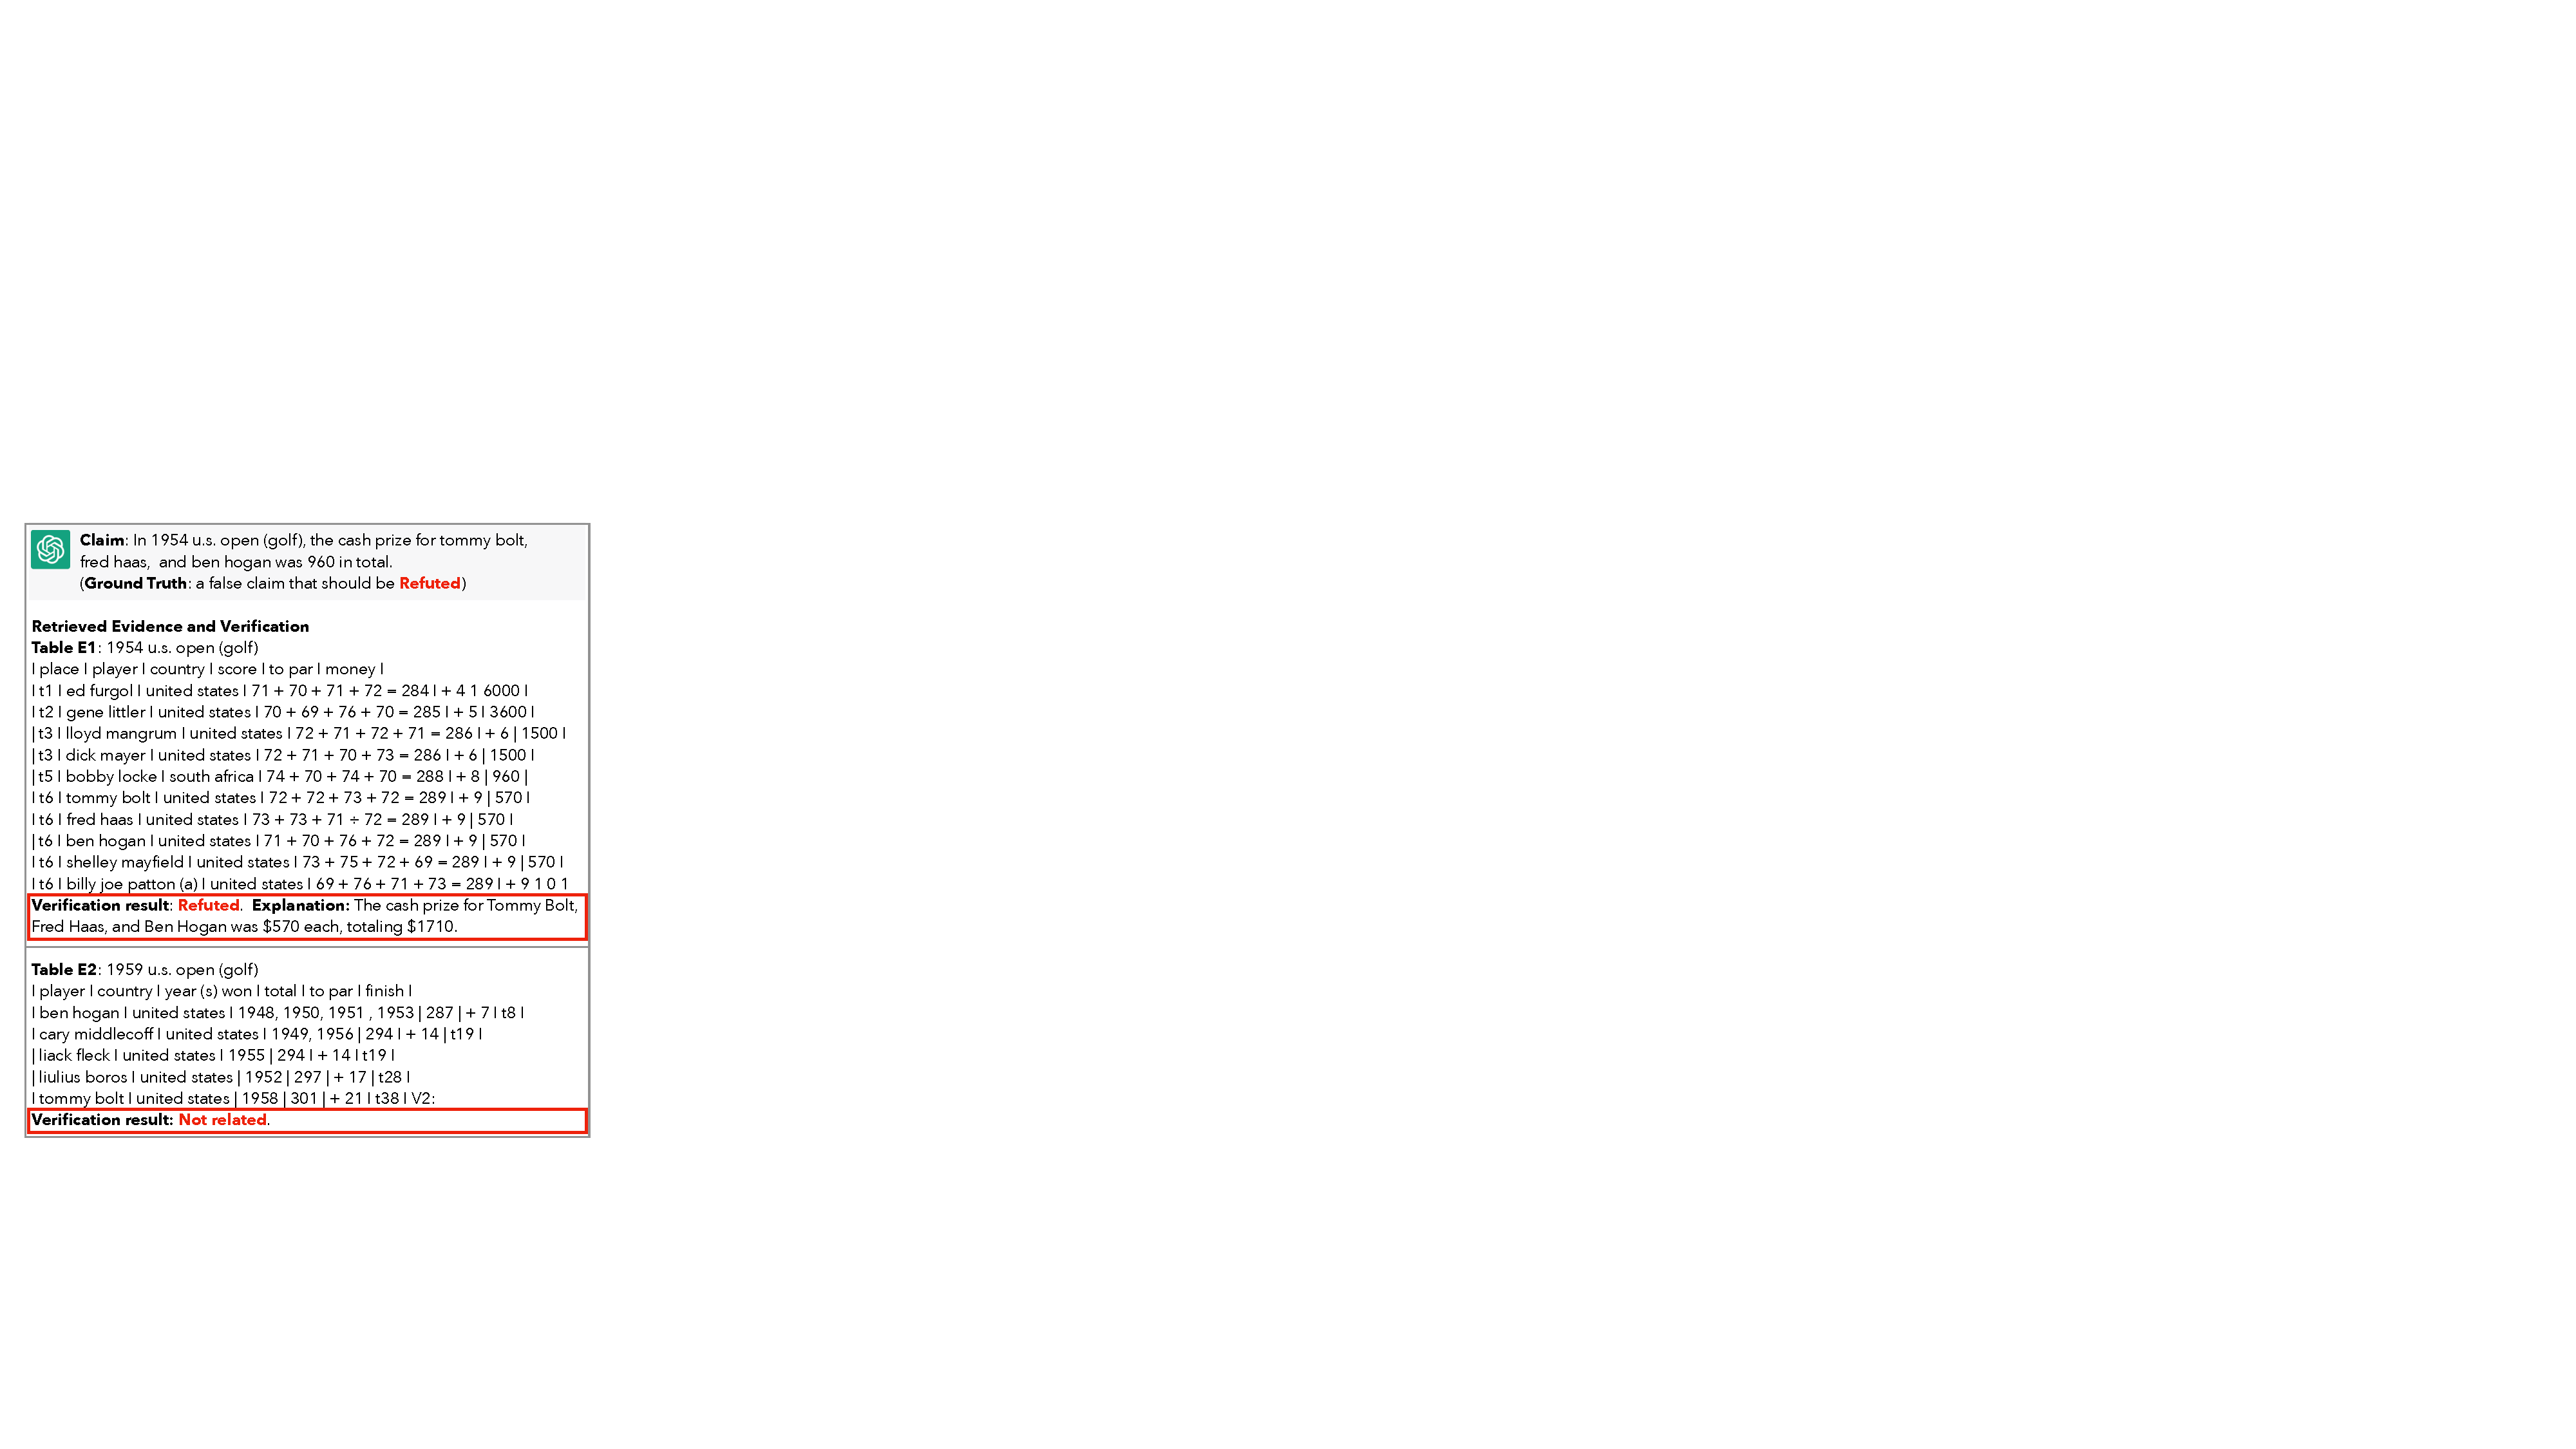
\includegraphics[width=0.65\textwidth]{submissions/Nan2024/figs/tabfact.pdf}
  \caption{Verifying a textual claim using retrieved tables.}
  \label{fig:claim_case} 
\end{center}
\end{figure}


\stitle{Evaluation for Retrieval.} 
We use Elasticsearch~\cite{elasticsearch} to retrieve the top-5 tables for each textual claim. Given the limited amount of relevant data, we focus on the recall metric for evaluation. Each textual claim is associated with a corresponding table in the original dataset, which we consider relevant evidence, while other retrieved tables are deemed irrelevant. The retrieval performance, measured by R@5, is 0.88.

\stitle{Evaluation for Verification.} 
We evaluate the verification process using two different verifiers: GPT-3.5, the default verifier for both data types, and PASTA~\cite{pasta}, a specialized model for text verification.
%
The performance of the verifiers is measured by accuracy. When the retrieved data cannot support or refute a claim, the verifier outputs ``not related''. However, in this case, since PASTA that only offers two different answers: ``true'' or ``false'', we consider it's also correct when PASTA outputs ``false''.

We conduct experiments in two settings. When a relevant table is retrieved and provided as evidence to the verifier, PASTA achieves higher accuracy than GPT-3.5 (0.89 vs. 0.75) in verifying the textual claim based on the table. However, in cases where many of the retrieved tables are irrelevant to the claim, the verifier must accurately determine which tables are not related. In this setting, PASTA's accuracy drops to 0.72 because it has not encountered this scenario during training, while GPT-3.5 improves to 0.91. 
% Thus, GPT-3.5-turbo demonstrates superior generalization capabilities and performs better than PASTA when dealing with irrelevant tables.
Thus, when the retrieved data is highly related to the generative data, local models like PASTA have higher accuracy while protecting privacy. In contrast, GPT-3.5 is better at generalizing and providing explanations for further judgments. Users can select the appropriate model based on their requirements.


In Figure~\ref{fig:claim_case}, we present a case of verifying a textual claim based on retrieved tables using GPT-3.5. \sys retrieves two tables $E_1$ and $E_2$, where $E_1$ can be used with an aggregation query to refute the claim while $E_2$ is not related because it is for the year 1959. The red boxes in Figure~\ref{fig:claim_case} show that GPT-3.5 can provide not only a verification result but also some explanation.






\section{Concluding Remarks}
\label{sec:discussion}
In this paper, we reconcile efficiency and security for uplink communication in Federated Learning. 
We propose to adapt existing compression mechanisms such as scalar quantization and pruning to the secure aggregation protocol by imposing a linearity constraint on the decompression operator. 
Our experiments demonstrate that we can adapt both quantization and pruning mechanisms to obtain a high degree of uplink compression with minimal degradation in performance and higher security guarantees. For achieving the highest rates of compression, we introduce \SecInd, a variant of \SecAgg well-suited for TEE-based implementation that supports product quantization while maintaining a high security bar. 
%We plan to extend our work to other federated learning scenarios, such as asynchronous FL, and further investigate the interaction of compression and privacy.
%\section{Extensions} 
As mentioned in Section~\ref{sec:intro}, we {may want } both \SecAgg and Differential Privacy~\citep{abadi2016deep} to realize the full promise of FL as a privacy-enhancing technology. 
While our primary focus is on enabling efficient and secure uplink communication, we emphasize that the proposed approaches are compatible with user-level DP. 
For instance, {at the cost of increasing the complexity of the trusted computing base}, DP noise can be added natively by the TEE with our modified random pruning or scalar quantization approaches. 
For PQ  and \SecInd, {we can have the TEE to add noise in the assignment space (\ie outputting a noisy histogram), or to map the histogram to the codeword space and add noise there.
Each option offers a different tradeoff between privacy, trust, and accuracy; we leave detailed evaluation to future work.}




%\modif{\textbf{Compatibility with DP.} 
%\sout{it would require, however, to transfer the aggregation to TEE or to design a DP mechanism in the assignment space, since DP noise must be added by the TEE and not by the server.}}

%\modif{\textbf{Efficiency and Privacy.}} A separate line of work {aims} to combine communication efficiency and privacy. 
%For instance, \cite{triastcyn2021dprec} develop a method that unifies compressed communication and DP (where integration with \SecAgg is left as an open problem), while \cite{chaudhuri2022privacyaware} design a privacy-aware scalar compression mechanism within the \emph{local} differential privacy model.

%\graham{\sout{
%\modif{\textbf{Broader Social Impact. }} In this work, we propose to enhance the privacy of individuals who may contribute to training ML models and simultaneously enable more individuals to participate in private training, who might otherwise have been excluded due to resource constraints. }}
% Indeed, Federated Learning could enable a malicious server to access individual model updates that can leak personal information. Hence, we propose a secure way to communicate the individual model updates.

% - Generic and less data-dependent codebook
% - Model compression 
% - Compression and DP
% - Error correction

% There are multiple extensions of PQ, such as having multiple codebooks per matrix  (which increases the cost of storing the codebooks) or performing the assignments with other norms than the $L_2$ norm.



% As a side note, \cite{jia2022federated} propose to perform domain adaptation by fine-tuning a small fraction of the model parameters, which is naturally compatible with Secure Aggregation, but requires to start from a pretrained model. 


\section{Conclusion}
In this paper, we reconcile efficiency and security for uplink communication in Federated Learning. We propose to adapt existing compression mechanisms such as scalar quantization and pruning to the secure aggregation protocol by imposing a linearity constraint on the decompression operator. Our experiments demonstrate that we can adapt both quantization and pruning mechanisms to obtain a high degree of uplink compression with minimal degradation in performance and higher security guarantees. For achieving the highest rates of compression, we introduce \SecInd, a variant of \SecAgg well-suited for TEE-based implementation that supports product quantization while maintaining a high security bar. 
We plan to extend our work to other federated learning scenarios, such as asynchronous FL, and further investigate the interaction of compression and privacy.
% and global and local differential privacy, 
% and investigate strategies to select optimal compression parameters 
% (quantization scales, centroids and pruning masks) 
% for better performance in these scenarios.

% % This 
% % - Generic and less data-dependent codebook
% % - Model compression 
% % - Compression and DP
% % - Error correction

% % \section*{Acknowledgements}


\bibliography{bibliography}
\bibliographystyle{plainnat}
% \pagebreak
\graham{\sout{Checklist}}
%\section*{Checklist}

% %%% BEGIN INSTRUCTIONS %%%
% The checklist follows the references.  Please
% read the checklist guidelines carefully for information on how to answer these
% questions.  For each question, change the default \answerTODO{} to \answerYes{},
% \answerNo{}, or \answerNA{}.  You are strongly encouraged to include a {\bf
% justification to your answer}, either by referencing the appropriate section of
% your paper or providing a brief inline description.  For example:
% \begin{itemize}
%   \item Did you include the license to the code and datasets? \answerYes{See Section~\ref{gen_inst}.}
%   \item Did you include the license to the code and datasets? \answerNo{The code and the data are proprietary.}
%   \item Did you include the license to the code and datasets? \answerNA{}
% \end{itemize}
% Please do not modify the questions and only use the provided macros for your
% answers.  Note that the Checklist section does not count towards the page
% limit.  In your paper, please delete this instructions block and only keep the
% Checklist section heading above along with the questions/answers below.
% %%% END INSTRUCTIONS %%%

\begin{enumerate}
\item For all authors...
\begin{enumerate}
  \item Do the main claims made in the abstract and introduction accurately reflect the paper's contributions and scope?
    \answerYes{See the claim list in Section~\ref{sec:intro}}
  \item Did you describe the limitations of your work?
    \answerYes{See in particular Section~\ref{sec:discussion}}
  \item Did you discuss any potential negative societal impacts of your work?
    \answerYes{See in particular Section~\ref{sec:discussion}}
  \item Have you read the ethics review guidelines and ensured that your paper conforms to them?
    \answerYes{}
\end{enumerate}


\item If you are including theoretical results...
\begin{enumerate}
  \item Did you state the full set of assumptions of all theoretical results?
    \answerNA{}
        \item Did you include complete proofs of all theoretical results?
    \answerNA{}
\end{enumerate}


\item If you ran experiments...
\begin{enumerate}
  \item Did you include the code, data, and instructions needed to reproduce the main experimental results (either in the supplemental material or as a URL)?
    \answerYes{We provide detailed instructions in Section~\ref{sec:experiments} and in the Appendix}  \answerNo{We did not provide the code in the supplementary but will provide it when publishing the paper} 
  \item Did you specify all the training details (e.g., data splits, hyperparameters, how they were chosen)?
    \answerYes{See Section~\ref{sec:experiments} and in the Appendix}
        \item Did you report error bars (e.g., with respect to the random seed after running experiments multiple times)?
    \answerYes{See Section~\ref{sec:experiments} in the setup description and Appendix for the detailed error bars over 3 independent runs. Note that we do not report bars for ablation results.}
        \item Did you include the total amount of compute and the type of resources used (e.g., type of GPUs, internal cluster, or cloud provider)?
    \answerYes{See Section~\ref{sec:experiments} in the setup description.}
\end{enumerate}


\item If you are using existing assets (e.g., code, data, models) or curating/releasing new assets...
\begin{enumerate}
  \item If your work uses existing assets, did you cite the creators?
    \answerYes{See Section~\ref{sec:experiments}}
  \item Did you mention the license of the assets?
    \answerYes{See Appendix}
  \item Did you include any new assets either in the supplemental material or as a URL?
    \answerNo{}
  \item Did you discuss whether and how consent was obtained from people whose data you're using/curating?
    \answerNA{}
  \item Did you discuss whether the data you are using/curating contains personally identifiable information or offensive content?
    \answerNA{}
\end{enumerate}


\item If you used crowdsourcing or conducted research with human subjects...
\begin{enumerate}
  \item Did you include the full text of instructions given to participants and screenshots, if applicable?
    \answerNA{}
  \item Did you describe any potential participant risks, with links to Institutional Review Board (IRB) approvals, if applicable?
    \answerNA{}
  \item Did you include the estimated hourly wage paid to participants and the total amount spent on participant compensation?
    \answerNA{}
\end{enumerate}


\end{enumerate}}


% %%%%%%%%%%%%%%%%%%%%%%%%%%%%%%%%%%%%%%%%%%%%%%%%%%%%%%%%%%%%%%%%%%%%%%%%%%%%%%%
% %%%%%%%%%%%%%%%%%%%%%%%%%%%%%%%%%%%%%%%%%%%%%%%%%%%%%%%%%%%%%%%%%%%%%%%%%%%%%%%
% % SUPPLEMENTAL CONTENT AS APPENDIX AFTER REFERENCES
% %%%%%%%%%%%%%%%%%%%%%%%%%%%%%%%%%%%%%%%%%%%%%%%%%%%%%%%%%%%%%%%%%%%%%%%%%%%%%%%
% %%%%%%%%%%%%%%%%%%%%%%%%%%%%%%%%%%%%%%%%%%%%%%%%%%%%%%%%%%%%%%%%%%%%%%%%%%%%%%%
\appendix
\appendix

\section{Datasets for FEL}
\label{sec:datasets}
In this section we would like to provide more details about our experiments. We first provide details about each dataset that was used. We then provide details about the model architectures that we used for each dataset.  


\subsection{Production Dataset}
Production dataset is an internal dataset that captures whether a user installs a mobile application after being shown a relevant advertisement item. A few hundred features are used as an input (the exact number cannot be disclosed) to predict a binary label (install/not-install). All the input features are public. For training, we use advertisement data from a random sample of 35 million users over a period of one month. Randomly selected 15 million users from the following week were used for testing.  

%\subsection{Open-Source Datasets}

\subsection{Taobao CTR Dataset}
The Taobao dataset contains 26 million interactions (click/non-click when an Ad was shown) between 1.14 million users and 847 thousand items across an 8-day period. 
The dataset uses 9 user features (e.g., gender or occupation), 6 item features (e.g., price or brand), and two contextual features (e.g., the day of week), which we assume to be all public to the service provider. 

In the Taobao CTR dataset, 16 out of the 17 features are sparse, with a categorical value encoding instead of a continuous, floating point value.
%
While server-based recommendation models use large embedding tables to convert these sparse features into a floating point embedding~\cite{din, dlrm, wideanddeep}, training such embedding tables on device is complicated because of the large memory capacity requirement (e.g., in the order of GB to TB~\cite{zhao2020distributed,acun:2021:understandingtraining,wilkening:2021:recssd,lui:2021:capacity}) and can leak private information more easily through gradients~\cite{alibaba_fl}. %significantly~\cite{zhang2021wide}.
Thus, we assume an architecture where embedding tables are pre-trained with opt-in users and are hosted on the server, while the rest of the model is trained with FEL using sparse features translated through the pre-trained tables. We randomly selected 10\% of the users as opt-in.

Note that our setup cannot achieve the accuracy that can be reached when we fully train the embedding tables, as we pre-train the embedding table and fix their weight during FL.
However, our setup represents a practical FL setup where training embedding tables on-device is prohibitive, due to client resource limitations~\cite{nguyen2021federated} and privacy concerns~\cite{alibaba_fl}.




\subsection{CelebA Smile Prediction Dataset}
While FEL is originally designed for recommendation and ranking tasks, we study its generality to non-recommendation models with CelebFaces Attributes Dataset (CelebA)~\cite{liu2015deep}. CelebA consists of $200,288$ images belonging to $9,343$ unique celebrities. Each image has 40 binary facial attribute annotations (e.g., bald, long hair, attractive, etc) and covers large pose variations and backgrounds.
We defined distinguishing between smiling/non-smiling images as our target task.

The Taobao dataset contains 26 million interactions (click/non-click when an Ad was shown) between 1.14 million users and 847 thousand items across an 8-day period. 
The dataset uses 9 user features (e.g., gender or occupation), 6 item features (e.g., price or brand), and two contextual features (e.g., the day of week), which we assume to be all public to the service provider. The details on how we preprocess the  dataset can be found in the appendix. 




\subsection{Model Architectures}
{\bf Production/Taobao Dataset:}
For recommendation datasets (production/Taobao CTR), we use a model that consists of 3 fully-connected hidden layers. The number of units at each hidden layer is decreasing exponentially with a parameter K. For instance, if $K=4$ and the input layer has 512 features, our neural network would have  $[512, 128, 32, 8, 1]$ neurons. For each dataset, we tune K to obtain a resulting model of approximately $10$MB. By doing so, it allows us to train a neural network even on older, low-tier devices with more limited memory capacity. ReLu is used as an activation function after each layer apart from the last one, where Sigmoid and binary cross-entropy was used.

For both datasets, we use synchronous FL with FedAvg~\cite{mcmahan2017learning}. We used the following hyperparameters for the Taobao dataset from an extensive hyperparameter search: client batch size of 32, 5 local epochs, 4096 clients per round, and a learning rate of 0.579 with SGD. Clients are selected at random and each only participates once (1 global epoch). The production dataset used similar hyperparameters.

For Taobao dataset's server-side pre-trained embedding table, we use an embedding dimension of 32, and train it with the 10\% opt-in users for 1 epoch using AdaGrad optimizer with learning rate of 0.01.

{\bf CelebA Dataset:}
For CelebA, we follow the setup of prior work~\cite{nguyen2021federated} and use a four layer CNN with dropout rate of 0.1, stride of 1, and padding of 2. We preprocess all images in train/validation/test sets; each image is resized and cropped to 32$\times$32 pixels, then normalized by 0.5 mean and 0.5 standard deviation. We use asynchronous FL with a client batch size of 32 samples, 1 local epoch, 30 global epochs, and a learning rate of 0.899 with SGD.

\section{Evaluation Methodology}
\label{sec:appendix-b}
Our evaluation aims to answer the following questions:

\begin{itemize}
    \item Can FEL improve the model prediction quality over vanilla FL? [Section~\ref{sec:prediction-quality}]
    \item How do different ensemble aggregation methods affect the model accuracy? [Section~\ref{sec:prediction-quality}]
    \item How do different clustering methods affect the model accuracy? [Section~\ref{sec:prediction-quality-clustering}]
    \item How does FEL affect privacy compared to vanilla FL? [Section~\ref{sec:privacy-eval}]
\end{itemize}

To answer these questions we used the three datasets presented in Section~\ref{sec:datasets}. To study recommendation and ranking tasks, we used a production dataset and an open-source, Taobao's Click-Through-Rate (CTR) prediction dataset~\cite{li2021novel}.
To study the effect of FEL on non-recommendation use-cases, we additionally studied the LEAF CelebA Smile Prediction dataset~\cite{liu2015deep}. More details about these datasets and their associated model architecture can be found in Section~\ref{sec:datasets}.


Both the FL baseline and the FEL leaf models used the same set of hyperparameters. 
The FL baseline is trained using all the available client data. In FEL, the client data is clustered, and one leaf model is trained for each cluster. We vary the number of clusters from 3--10 and evaluate different clustering methods.
When training the over-arch NN layer, a small subset of opt-in users is used.


\begin{table}
\small
\centering
\caption{\label{tab:clusterconfig} Explanation of different cluster methods in Figure~\ref{fig:eval0} (right).}
\begin{tabular}{|l||l|l|c|}
\hline
Dataset & Config & Feature & \# clusters \\ \hline\hline
\multirow{4}{*}{Production} & Clustering 1 & Age & 5\\
 & Clustering 2 & App & 5\\
 & Clustering 3 & Location & 4\\
 & Clustering 4 & Click ratio & 10\\\hline
\multirow{3}{*}{Taobao~\cite{taobao}} & Clustering 1 & Age & 7\\
 & Clustering 2 & Consumption & 4\\
 & Clustering 3 & City level & 5\\\hline
\multirow{3}{*}{CelebA~\cite{liu2015deep}} & Clustering 1 & \# Attributes & 3\\
 & Clustering 2 & K-means & 3\\
 & Clustering 3 & K-means & 5\\\hline
\end{tabular}\\
\end{table}

% %


%%%%%%%%%%%%%%%%%%%%%%%%%%%%%%%%%%%%%%%%%%%%%%%%%%%%%%%%%%%%%%%%%%%%%%%%%%%%%%%
%%%%%%%%%%%%%%%%%%%%%%%%%%%%%%%%%%%%%%%%%%%%%%%%%%%%%%%%%%%%%%%%%%%%%%%%%%%%%%%


\end{document}


% This document was modified from the file originally made available by
% Pat Langley and Andrea Danyluk for ICML-2K. This version was created
% by Iain Murray in 2018. It was modified from a version from Dan Roy in
% 2017, which was based on a version from Lise Getoor and Tobias
% Scheffer, which was slightly modified from the 2010 version by
% Thorsten Joachims & Johannes Fuernkranz, slightly modified from the
% 2009 version by Kiri Wagstaff and Sam Roweis's 2008 version, which is
% slightly modified from Prasad Tadepalli's 2007 version which is a
% lightly changed version of the previous year's version by Andrew
% Moore, which was in turn edited from those of Kristian Kersting and
% Codrina Lauth. Alex Smola contributed to the algorithmic style files.
